% Reconstructed semantic LaTeX: editable paragraphs, equations, figures and citations.

\chapter{Machine-learning methodology}
\label{sec:04_machine_learning_methodology_machine_learning_methodology}

\section{Machine-learning objectives and foundations}
\label{sec:04_machine_learning_methodology_machine_learning_objectives_and_foundations}

The models developed in this work are trained in a supervised setting from simulated input– output pairs. The inputs may include beam distributions, phase-space histograms, latent states, lattice-element descriptors, or machine parameters, while the targets correspond to evolved densities, reconstructed distributions, propagated latent states, or physical beam descriptors. Standard neural-network and variational-inference definitions used throughout this section are collected in Appendix A.1.

\subsection{From data to prediction}
\label{sec:04_machine_learning_methodology_from_data_to_prediction}

Given a dataset

\begin{equation}
\label{eq:55}
\mathcal D=\left\{\left(x^{(s)},y^{(s)}\right)\right\}_{s=1}^{N},
\end{equation}

a parameterized model \(f_{\theta} : \mathcal{X} \to \mathcal{Y}\) is trained by minimizing an empirical loss,

\begin{equation}
\label{eq:56}
\theta^{\star}=\underset{\theta}{\arg\min}\;\frac1N\sum_{s=1}^{N}\ell\left(f_{\theta}\left(x^{(s)}\right),y^{(s)}\right).
\end{equation}

During training, gradients obtained through backpropagation are used to update the model parameters. The complete workflow is summarized in Fig. 2.

\begin{figure}[!htbp]
\centering
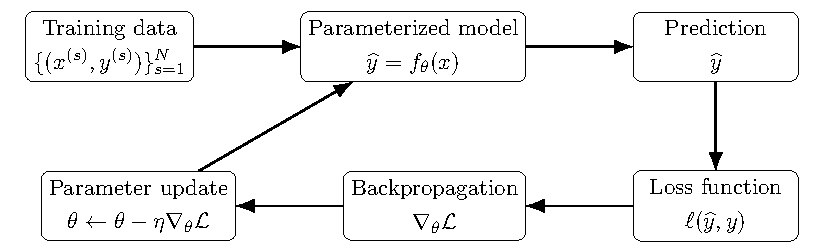
\includegraphics[width=0.8945\linewidth]{supervised_learning_workflow.pdf}
\caption{Basic supervised machine-learning workflow. Input examples are propagated through a parameterized model to obtain predictions. A loss function compares predictions with the ground-truth targets, and backpropagation provides gradients used to update the model parameters. After training, inference consists only of evaluating the learned forward map.}
\label{fig:supervised_learning_workflow}
\end{figure}

Once training is complete, the optimization loop is removed and inference consists only of evaluating

\begin{equation}
\label{eq:57}
\widehat y_{\mathrm{new}}=f_{\theta^{\star}}(x_{\mathrm{new}}).
\end{equation}

The purpose of the surrogate models developed in this work is to make this forward evaluation substantially cheaper than rerunning the corresponding reference simulation.

\subsection{Neural-network building blocks}
\label{sec:04_machine_learning_methodology_neural_network_building_blocks}

Dense layers are used throughout the models to transform global variables such as machine parameters, physical beam descriptors, and latent states. They apply learned affine transformations followed by nonlinear activation functions, allowing the networks to represent nonlinear input–output relations.

Convolutional layers are used for the projected beam distributions. Each six-dimensional beam cloud is represented by its fifteen pairwise two-dimensional histograms,

\begin{equation}
\label{eq:58}
X=H(\rho)\in\mathbb R^{15\times N_b\times N_b}.
\end{equation}

Shared convolutional kernels exploit the local organization of these histograms and can identify structures such as compact cores, asymmetries, tails, filamentation, and halo. Successive convolutional and downsampling layers compress the distributions into learned features, while the decoder reverses this process to reconstruct the projected beam state.

\subsection{Conditional variational latent representation}
\label{sec:04_machine_learning_methodology_conditional_variational_latent_representation}

Directly propagating all fifteen \(N_{b} \times N_{b}\) histograms through the accelerator lattice would be computationally expensive. The beam representation is therefore compressed using a conditional variational autoencoder (CVAE). The encoder maps the distributions and conditioning variables to a probabilistic latent state,

\begin{equation}
\label{eq:59}
q_{\phi}(z\mid X,c),
\end{equation}

and the decoder reconstructs the distributions through

\begin{equation}
\label{eq:60}
p_{\psi}(X\mid z,c).
\end{equation}

The latent state retains a compact representation of the projected beam shape, while variational regularization produces a structured latent space that can be sampled and propagated. The complete CVAE architecture and its training objective are introduced in Section 4.6.

The normalized histograms do not retain all information about the physical position and extension of the beam. The representation therefore also includes six coordinate centroids and six coordinate-wise RMS spreads,

\begin{equation}
\label{eq:61}
\begin{gathered}\mathbf m=(\langle x\rangle,\langle p_x\rangle,\langle y\rangle,\langle p_y\rangle,\langle\zeta\rangle,\langle\delta\rangle),\\\boldsymbol\sigma=(\sigma_x,\sigma_{p_x},\sigma_y,\sigma_{p_y},\sigma_{\zeta},\sigma_{\delta}),\end{gathered}
\end{equation}

combined into

\begin{equation}
\label{eq:62}
\mathbf a=[\mathbf m,\boldsymbol\sigma]\in\mathbb R^{12}.
\end{equation}

For a projected plane \(( \xi_{i} , \xi_{j} ) ,\) its physical axes are determined by the shared descriptors \(( m_{i} , \sigma_{i} , m_{j} , \sigma_{j} ) .\) The model therefore separates normalized distributional shape, represented in latent space, from physical position and extension, represented explicitly by the statistical descriptors.

\section{Operator-learning formulation}
\label{sec:04_machine_learning_methodology_operator_learning_formulation}

The beam-dynamics problems introduced in the preceding sections are naturally formulated at the level of functions and probability densities. In the absence of collective effects, a phase-space density is transported by the pushforward of a single-particle map. Once self-consistent forces, wakefields, damping, or diffusion are included, however, the evolution becomes a generally nonlinear transformation acting on the distribution itself. The learning problem is therefore more naturally posed as the approximation of an operator rather than as conventional finite-dimensional regression. This would allow to learn different lattice configurations, collective-effect parameters, and initial conditions within a single model.

Let \(A\) and \(U\) denote suitable spaces of input and output functions, densities, or reduced beam representations, and let

\begin{equation}
\label{eq:63}
\mathcal M\subset\mathbb R^m
\end{equation}

denote the admissible machine-parameter domain. The physical target is an operator

\begin{equation}
\label{eq:64}
\mathcal G^{\dagger}:\mathcal A\times\mathcal M\longrightarrow\mathcal U,\qquad(a,\mu)\longmapsto u,
\end{equation}

where \(a \in A\) denotes the input state, \(u \in U\) the output state, and \(\mu \in \mathcal{M}\) contains machine or collective-effect parameters.

Given \(\mathcal{D} ,\) the set of physical observations corresponding to the operator \(\mathcal{G}^{\dagger} ,\)

\begin{equation}
\label{eq:65}
\mathcal D=\left\{\left(a^{(s)},\mu^{(s)},u^{(s)}\right)\right\}_{s=1}^{N},
\end{equation}

the empirical objective is to approximate \(\mathcal{G}^{\dagger}\) by a parameterized family \(\mathcal{G}_{\theta} ,\)

\begin{equation}
\label{eq:66}
\theta^{\star}=\underset\theta{\arg\min}\;\frac1N\sum_{s=1}^{N}\left\|\mathcal G_{\theta}\left(a^{(s)},\mu^{(s)}\right)-u^{(s)}\right\|_{\mathcal U}^{2}.
\end{equation}

The choice of norm depends on the physical object being learned. A discrete \(L^{2}\) loss is a natural choice for smooth density profiles \cite{kovachki2023operators}. Sobolev-type objectives additionally penalize discrepancies in derivatives and are therefore useful when gradient information or fine-scale structure is relevant \cite{adams2003sobolev}. Low-order moment penalties can directly constrain physically meaningful quantities such as centroids and coordinate-wise RMS spreads, whereas optimal-transport discrepancies account for the geometric displacement of probability mass and are consequently well suited to comparing spatial probability distributions \cite{peyre2019transport}.

This formulation is particularly important for the present work because the different machine-learning models do not necessarily operate on the same discretized representation. The longitudinal FNO acts directly on gridded line densities, whereas the six-dimensional models act on compressed representations of projected phase-space densities. Nevertheless, both can be interpreted as approximations of physical evolution operators at different levels of description.

\section{Neural operators}
\label{sec:04_machine_learning_methodology_neural_operators}

\subsection{From kinetic equations to solution operators}
\label{sec:04_machine_learning_methodology_from_kinetic_equations_to_solution_operators}

The motivation for neural operators becomes clearer by returning to the governing equations. At the kinetic level, collective beam dynamics are commonly described using the Vlasov equation, or the Vlasov–Fokker–Planck equation when damping and diffusion are included \cite{wiedemann2015vlasov,metral2022mitigation,schoenfeldt2017vfp}. A generic collective beam-density evolution may therefore be written schematically as

\begin{equation}
\label{eq:67}
\partial_s\rho+\nabla_{\xi}\cdot[\mathbf F_{\mathrm{ext}}(\xi,s,\mu)\rho]+\nabla_{\xi}\cdot[\mathbf F_{\mathrm{coll}}[\rho](\xi,s,\mu)\rho]=\mathcal D_{\mu}[\rho],
\end{equation}

where

\begin{equation}
\label{eq:68}
\xi=(x,p_x,y,p_y,\zeta,\delta)\in\mathbb R^6
\end{equation}

denotes the six-dimensional phase-space coordinate, \(F_{\mathrm{ext}}\) is the external lattice force, \(F_{\mathrm{coll}} [ \rho ]\) is a density-dependent collective force, and \(\mathcal{D}^{\mu} [ \rho ]\) represents dissipative or diffusive effects.

Equation~\eqref{eq:67} may be written abstractly as

\begin{equation}
\label{eq:69}
\partial_s\rho=\mathcal L_{\mu}[\rho],
\end{equation}

where \(\mathcal{L}_{\mu}\) denotes the generally nonlinear kinetic generator. For suitable initial data \(\rho_{0} ,\) the corresponding evolution defines a parameter-dependent solution operator

\begin{equation}
\label{eq:70}
\mathcal S_s^{\mu}:\rho_0\longmapsto\rho_s.
\end{equation}

Equivalently, over a finite propagation step \(\Delta s ,\) the solution operator may be written as

\begin{equation}
\label{eq:71}
\rho_{s+\Delta s}=\mathcal S_{\Delta s}^{\mu}[\rho_s].
\end{equation}

This distinction is fundamental. A classical numerical solver approximates the solution of the governing equation for each new initial condition and parameter choice. An operator-learning model instead attempts to approximate the map

\begin{equation}
\label{eq:72}
(\rho_s,\mu)\longmapsto\rho_{s+\Delta s}
\end{equation}

over a family of admissible initial states and machine configurations.

The same perspective applies to reduced longitudinal collective dynamics. The induced wake potential is already an integral operator acting on the bunch profile,

\begin{equation}
\label{eq:73}
V_{\parallel}(z)=\int_{-\infty}^{\infty}W_{\parallel}(z-z')\lambda(z')\,\mathrm dz'.
\end{equation}

Thus,

\begin{equation}
\label{eq:74}
\mathcal W:\lambda\longmapsto V_{\parallel}
\end{equation}

is a functional map whose kernel is the wake function.

Likewise, the Haïssinski problem defines a nonlinear self-consistent relation between the bunch density and its induced field. If \(\mathcal{H}\) denotes the nonlinear update associated with the stationary equation, the equilibrium profile satisfies \cite{funkner2025wake}

\begin{equation}
\label{eq:75}
\lambda_h=\mathcal H[\lambda_h;W,I,\mu].
\end{equation}

The equilibrium density is therefore a fixed point of a nonlinear operator. One may consequently seek to learn either the fixed-point solution map

\begin{equation}
\label{eq:76}
\mathcal G_{\mathrm H}^{\dagger}:(W,I,\mu)\longmapsto\lambda_h,
\end{equation}

or a finite-step relaxation operator

\begin{equation}
\label{eq:77}
\mathcal G_{\Delta k}^{\dagger}:(\lambda^{(k)},\mu)\longmapsto\lambda^{(k+\Delta k)}.
\end{equation}

At the full kinetic level, an analogous target is

\begin{equation}
\label{eq:78}
\mathcal G_t^{\dagger}:(\rho_0,\mu)\longmapsto\rho_t,
\end{equation}

which approximates the evolution generated by a Vlasov–Fokker–Planck-type equation.

From this perspective, it is clear that collective beam dynamics is naturally an operator-learning problem. The target is not merely the value of a scalar observable at one point, but the transformation of an entire density, field, or functional representation under parameter-dependent physical dynamics.

\subsection{General neural-operator architecture}
\label{sec:04_machine_learning_methodology_general_neural_operator_architecture}

Neural operators are parameterized models designed to approximate maps between function spaces. Following the general framework described by Kovachki et al.\cite{kovachki2023operators}, the continuous object of interest is

\begin{equation}
\label{eq:79}
\mathcal G^{\dagger}:\mathcal A\longrightarrow\mathcal U,
\end{equation}

where \(\mathcal{A}\) and \(\mathcal{U}\) are suitable function spaces, typically Banach spaces of scalar- or vector-valued fields \cite{kovachki2023operators}.

Given an input field \(a ( x ) ,\) the lifting stage is written as

\begin{equation}
\label{eq:80}
v_0(x)=\mathcal P\bigl(a(x),x,\mu\bigr),
\end{equation}

where \(P\) is generally a pointwise neural network. The explicit inclusion of the coordinate \(x\) allows the model to retain information about domain geometry, while \(\mu\) provides parametric dependence on machine or beam settings.

The latent field is then propagated through \(T\) operator layers\cite{arpaia2021machine},

\begin{equation}
\label{eq:81}
v_{t+1}(x)=\sigma\bigl(W_tv_t(x)+\mathcal K_{\theta,t}[v_t](x)+b_t(x)\bigr),\quad t=0,\ldots,T-1,
\end{equation}

where \(W_{t}\) is a local linear transformation, \(b_{t}\) is a bias, \(\sigma\) a pointwise nonlinearity, and \(\mathcal{K}_{\theta , t}\) a learned nonlocal operator.

For an integral-kernel parameterization,

\begin{equation}
\label{eq:82}
\mathcal K_{\theta,t}[v_t](x)=\int_D\kappa_{\theta,t}(x,y,\mu)v_t(y)\,\mathrm d\nu(y),
\end{equation}

so that

\begin{equation}
\label{eq:83}
v_{t+1}(x)=\sigma\left(W_tv_t(x)+\int_D\kappa_{\theta,t}(x,y,\mu)v_t(y)\,\mathrm d\nu(y)+b_t(x)\right).
\end{equation}

Here, \(\kappa_{\theta , t} ( x , y , \mu )\) is the learned kernel and \(\nu\) is the measure associated with the domain discretization.

Finally, a projection map produces the output field,

\begin{equation}
\label{eq:84}
u(x)=\mathcal Q(v_T(x)).
\end{equation}

This formulation is particularly relevant to collective beam physics. The local term \(W_{t} v_{t} ( x )\) can represent pointwise or local corrections, while the kernel term

\begin{equation}
\label{eq:85}
\int_D\kappa_{\theta,t}(x,y)v_t(y)\,\mathrm d\nu(y)
\end{equation}

represents structured nonlocal interactions. Such a decomposition is conceptually compatible with beam dynamics, where local lattice transport coexists with nonlocal collective interactions generated by wakefields and self-consistent fields.

The architecture should not, however, be interpreted as automatically enforcing the governing equations. Unless physical constraints are inserted explicitly, the learned kernel remains data driven. The advantage is instead one of representation as the model class is constructed to approximate operators acting on fields and distributions in functional spaces emerging form underlying parametrized differential equations, rather than only maps between fixed finite-dimensional vectors.

\subsection{Discretization and approximation}
\label{sec:04_machine_learning_methodology_discretization_and_approximation}

One of the central motivations for neural operators is that the model is conceptually defined at the level of functions rather than at the level of one fixed coordinate vector. In the theoretical neural-operator framework, the parameterization can be constructed so that its number of learned parameters does not depend directly on the number of discretization points \cite{kovachki2023operators}.

This property is especially relevant in accelerator modelling, where the same underlying density may be represented using different, longitudinal grid resolutions, histogram bin numbers, macroparticle populations, spectral truncations, or observation meshes. A discretization-invariant architecture allows the same learned operator to be applied to different representations of the same underlying physical state.

Nevertheless, cross-resolution transfer should be interpreted carefully. A discretization-invariant architecture does not imply that predictions are automatically identical on arbitrary meshes or that no numerical error is introduced by changing resolution. Rather, the continuous operator and its discrete realization must be distinguished.

Let \(D_{L}\) denote a discretization with resolution parameter \(L ,\) and let \(\mathcal{G}_{\theta} b\) denote the numerical realization of the continuous learned operator \(\mathcal{G}_{\theta} .\) Then

\begin{equation}
\label{eq:86}
\begin{aligned}\left\|\widehat{\mathcal G}_{\theta}(D_L,a|_{D_L})-\mathcal G^{\dagger}(a)\right\|_{\mathcal U}&\le\underbrace{\left\|\widehat{\mathcal G}_{\theta}(D_L,a|_{D_L})-\mathcal G_{\theta}(a)\right\|_{\mathcal U}}_{\text{discretization error}}\\&\quad+\underbrace{\left\|\mathcal G_{\theta}(a)-\mathcal G^{\dagger}(a)\right\|_{\mathcal U}}_{\text{approximation error}}.\end{aligned}
\end{equation}

For the present discussion in beam dynamics, the target operator may describe either non-collective transport or evolution including collective self-interactions. This distinction can be made explicit by writing the beam-density equation as

\begin{equation}
\label{eq:87}
\partial_s\rho=\mathcal L_{\mathrm{ext}}^{\mu}\rho+\lambda\mathcal N_{\mathrm{coll}}^{\mu}[\rho],
\end{equation}

where

\begin{equation}
\label{eq:88}
\mathcal L_{\mathrm{ext}}^{\mu}\rho=-\nabla_{\xi}\cdot[\mathbf F_{\mathrm{ext}}(\xi,s,\mu)\rho]+\mathcal D_{\mu}[\rho],
\end{equation}

and

\begin{equation}
\label{eq:89}
\mathcal N_{\mathrm{coll}}^{\mu}[\rho]=-\nabla_{\xi}\cdot[\mathbf F_{\mathrm{coll}}[\rho](\xi,s,\mu)\rho].
\end{equation}

Here, \(\lambda\) controls the strength of the collective interaction. For example, it may represent an impedance or wakefield scaling factor.

When \(\lambda =\) 0, particles evolve under the prescribed external lattice without modifying the force acting on the rest of the beam. In the Hamiltonian limit, this evolution is described by a symplectic single-particle map \cite{huang2024symplectic}. The particle trajectories may still be nonlinear functions of the phase-space coordinates because of nonlinear lattice elements. Nevertheless, provided that \(\mathcal{D}^{\mu}\) is linear, the corresponding density propagator \(\mathcal{G}_{0}^{\dagger}\) remains linear with respect to the input density,

\begin{equation}
\label{eq:90}
\mathcal G_0^{\dagger}(\alpha\rho_1+\beta\rho_2;\mu)=\alpha\mathcal G_0^{\dagger}(\rho_1;\mu)+\beta\mathcal G_0^{\dagger}(\rho_2;\mu).
\end{equation}

When \(\lambda \not =\) 0, the force depends on the evolving beam density through wakefields, impedances, space charge, or other collective mechanisms \cite{metral2021wake,ghribi2026collective}. The resulting propagator \(\mathcal{G}_{\lambda}^{\dagger}\) is therefore generally nonlinear in \(\rho .\) Even when the collective force is obtained from a linear convolution of the density with a wake function, the product \(F_{\mathrm{coll}} [ \rho ] \rho\) makes the density evolution nonlinear and typically nonlocal.

This distinction also clarifies the role of the two errors in Eq.~\eqref{eq:86}. In the non-collective regime, discretization error arises principally from representing and transporting the phase-space density on a finite grid or with a finite macroparticle sample. In the collective regime, an inaccurate density representation also perturbs the computed self-consistent force, and this error is fed back into the subsequent evolution. Insufficient resolution of narrow structures, tails, or longitudinal modulations can therefore alter both the represented density and the collective force generated by that density. Cross-resolution transfer is consequently a more demanding test in the collective regime. Increasing the number of bins may reduce this error only when the associated macroparticle sampling noise remains controlled.

A direct comparison between the two regimes may be expressed through the collective correction

\begin{equation}
\label{eq:91}
\Delta\rho_{\mathrm{coll}}(s)=\mathcal G_{\lambda}^{\dagger}(\rho_0;\mu)-\mathcal G_0^{\dagger}(\rho_0;\mu),
\end{equation}

obtained by propagating the same initial density and external lattice with and without collective interactions. A learned operator conditioned on \(\lambda\) may approximate both regimes, while Eq.~\eqref{eq:91} isolates the density modification attributable to collective effects.

Under appropriate assumptions, neural-operator classes satisfy universal-approximation results for continuous operators on compact subsets of function spaces \cite{kovachki2023operators}. Such results provide theoretical motivation for the framework, but they do not remove the practical requirements of representative data, stable optimization, adequate discretization, and physically meaningful validation.

The central kernel operator

\begin{equation}
\label{eq:92}
\mathcal K_{\theta}[v](x)=\int_D\kappa_{\theta}(x,y)v(y)\,\mathrm d\nu(y)
\end{equation}

can be parameterized in several ways. The choice of parameterization determines the inductive bias, computational complexity, and geometry of the learned interaction.

A direct kernel parameterization leads to Graph Neural Operator-type models, in which the integral is approximated over sampled points or graph neighborhoods. A low-rank operator imposes a factorized representation of the kernel. Hierarchical variants introduce multi-scale interaction structures. On regular grids, a Fourier Neural Operator instead represents the kernel action in spectral space.

These models approximate different operators and act on different representations, but they arise from the same conceptual framework. The FNO parameterizes nonlocal interaction through spectral multipliers, whereas the GNO parameterizes it through a learned kernel evaluated over graph neighborhoods.

This common interpretation will later be important when comparing the GNO with the local-window Transformer. Although attention and graph message passing are different computational mechanisms, both can be interpreted as learned interaction kernels with different support constraints.

\section{Fourier Neural Operator}
\label{sec:04_machine_learning_methodology_fourier_neural_operator}

For reduced longitudinal problems defined on a regular grid, the Fourier Neural Operator provides a natural specialization of the general architecture. The starting point is the kernel operator

\begin{equation}
\label{eq:93}
\mathcal K_{\theta}[v](x)=\int_D\kappa_{\theta}(x,y)v(y)\,\mathrm dy.
\end{equation}

If the kernel is translation invariant,

\begin{equation}
\label{eq:94}
\kappa_{\theta}(x,y)=\kappa_{\theta}(x-y),
\end{equation}

the integral becomes a convolution,

\begin{equation}
\label{eq:95}
\mathcal K_{\theta}[v]=\kappa_{\theta}*v.
\end{equation}

By the convolution theorem,

\begin{equation}
\label{eq:96}
\mathcal F(\mathcal K_{\theta}[v])(k)=\mathcal F(\kappa_{\theta})(k)\mathcal F(v)(k).
\end{equation}

The FNO replaces the explicit Fourier transform of the kernel by a learned spectral multiplier

\begin{equation}
\label{eq:97}
\mathcal K_{\theta}v=\mathcal F^{-1}(R_{\theta}(k)\mathcal F(v)(k)).
\end{equation}

A complete FNO layer therefore takes the form

\begin{equation}
\label{eq:98}
v_{\ell+1}(x)=\sigma\left(W_{\ell}v_{\ell}(x)+\mathcal F^{-1}\bigl(R_{\theta,\ell}(k)\mathcal F(v_{\ell})(k)\bigr)(x)+b_{\ell}(x)\right).
\end{equation}

In practice, only a finite set of Fourier modes is retained. If \(K_{\mathrm{max}}\) denotes the maximum retained mode,

\begin{equation}
\label{eq:99}
\widehat v(k)=\mathcal F(v)(k),\qquad|k|\le K_{\max},
\end{equation}

then the spectral branch acts as

\begin{equation}
\label{eq:100}
\widehat{\mathcal K_{\theta}v}(k)=R_{\theta}(k)\widehat v(k),\qquad|k|\le K_{\max}.
\end{equation}

Modes outside the retained range do not pass through the learned spectral multiplier and are either truncated or represented indirectly through the local branch and nonlinear layer composition.

The computational appeal of this construction comes from the use of FFT-based transforms on uniform grids. For a grid containing \(N_{g}\) points, the Fourier transforms scale approximately as

\begin{equation}
\label{eq:101}
\mathcal O(N_g\log N_g),
\end{equation}

up to channel dimensions and spectral-mode multiplication costs.

The FNO is particularly appropriate for the longitudinal collective-effects problem because the underlying physics already possesses a spectral formulation. The induced voltage satisfies

\begin{equation}
\label{eq:102}
V_{\mathrm{ind}}(z)=-\mathcal F^{-1}\left[Z_{\parallel}(\omega)\widehat\lambda(\omega)\right](z),
\end{equation}

which has the same mathematical structure as multiplication by a spectral response followed by inverse transformation.

This does not imply that the learned multiplier \(R_{\theta} ( k )\) is identical to the physical impedance \(Z_{\Vert} ( \omega ) .\) The FNO is trained to approximate the complete target operator represented in the data, which may include nonlinear relaxation, RF confinement, parameter dependence, discretization effects, and several successive physical transformations. Nevertheless, the spectral architecture introduces an inductive bias consistent with the convolutional and frequency-domain structure of longitudinal collective interactions.

In the present work, the primary reduced FNO task is to learn the evolution of the longitudinal density under collective effects, parametrized by a vector \(\mu\) containing the physical parameters controlling the simulated collective response. For stationary problems, a second possible formulation is to learn the fixed-point map where the target is the self-consistent Haïssinski equilibrium. A third formulation acts directly on the collective field, where the target is the induced voltage or wake potential, which is the closest learned analogue of the physical wake-convolution operator.

These distinct formulations emphasize an important methodological point in operator learning. It does not prescribe a unique surrogate target, instead the methodology is defined depending on the intended application, one may learn the evolved density, the stationary solution, the collective field, or reduced observables. The experiments presented later focus on the mappings supported by the available simulation datasets, while the broader formulations define natural extensions of the present work.

\section{Graph Neural Operator}
\label{sec:04_machine_learning_methodology_graph_neural_operator}

The Fourier Neural Operator provides an efficient parameterization of nonlocal operators on regular grids. However, its spectral construction becomes less convenient when the underlying domain is irregular or nonuniformly sampled, when fine-scale structures require the retention of many higher Fourier harmonics, or when a high-dimensional domain makes the tensor-product spectral representation computationally expensive. Moreover, some physical systems are more naturally represented as sets of interacting elements rather than as fields on regular grids. In these settings, a Graph Neural Operator (GNO) provides an alternative discretization of the generic kernel operator introduced in Section 4.3. Rather than representing the kernel action in Fourier space, the GNO approximates the integral operator by evaluating learned interactions directly between sampled points or graph nodes \cite{li2020graph,kovachki2023operators}.

Starting from the continuous operator layer

\begin{equation}
\label{eq:103}
\mathcal K_{\theta}[v](x)=\int_D\kappa_{\theta}(x,y,\mu)v(y)\,\mathrm d\nu(y),
\end{equation}

let

\begin{equation}
\label{eq:104}
X=\{x_i\}_{i=1}^{N}
\end{equation}

be a discrete set of nodes sampling the domain (D). A quadrature approximation of Eq.~\eqref{eq:103} gives

\begin{equation}
\label{eq:105}
\mathcal K_{\theta}[v](x_i)\approx\sum_{j=1}^{N}\omega_{ij}\kappa_{\theta}(x_i,x_j,\mu)v(x_j),
\end{equation}

where \(\omega_{j}\) denotes a quadrature weight associated with node \(x_{j} .\) When interactions are restricted to a neighborhood \(\mathcal{N} ( i )\) of node \(i ,\) the discrete operator becomes

\begin{equation}
\label{eq:106}
\mathcal K_{\theta}[v](x_i)\approx\sum_{j\in\mathcal N(i)}\omega_{ij}\kappa_{\theta}(x_i,x_j,\mu)v(x_j).
\end{equation}

The neighborhood definition therefore determines the support of the learned interaction kernel.

A complete GNO layer may be written as

\begin{equation}
\label{eq:107}
v_i^{(\ell+1)}=\sigma\left(W_{\ell}v_i^{(\ell)}+\sum_{j\in\mathcal N(i)}\omega_{ij}\kappa_{\theta,\ell}(x_i,x_j,v_i^{(\ell)},v_j^{(\ell)},\mu)v_j^{(\ell)}+b_{\ell}\right),
\end{equation}

where \(W_{\ell}\) is a local linear transformation, \(\kappa_{\theta , \ell}\) is a learned kernel, \(\sigma\) is a nonlinear activation, and \(b_{\ell}\) is a bias term.

Equivalently, the operator can be expressed in message-passing form. Defining an edge message

\begin{equation}
\label{eq:108}
m_{ij}^{(\ell)}=\varphi_{\theta,\ell}(v_i^{(\ell)},v_j^{(\ell)},e_{ij},\mu),
\end{equation}

where \(e_{i j}\) contains relative geometric or physical information associated with the interaction between nodes \(i\) and \(j ,\) the aggregated message is

\begin{equation}
\label{eq:109}
m_i^{(\ell)}=\sum_{j\in\mathcal N(i)}m_{ij}^{(\ell)},
\end{equation}

and the node update becomes

\begin{equation}
\label{eq:110}
v_i^{(\ell+1)}=\psi_{\theta,\ell}(v_i^{(\ell)},m_i^{(\ell)}).
\end{equation}

This representation makes explicit that graph message passing is a discrete approximation of a learned integral operator rather than merely a generic graph-processing mechanism.

The distinction with the FNO is therefore primarily a distinction in kernel parameterization. The FNO evaluates a global translation-compatible interaction through spectral multiplication,

\begin{equation}
\label{eq:111}
\mathcal K_{\theta}^{\mathrm{FNO}}v=\mathcal F^{-1}(R_{\theta}(k)\mathcal F(v)(k)),
\end{equation}

whereas the GNO evaluates interactions directly between sampled locations,

\begin{equation}
\label{eq:112}
\mathcal K_{\theta}^{\mathrm{GNO}}v(x_i)=\sum_{j\in\mathcal N(i)}\omega_{ij}\kappa_{\theta}(x_i,x_j,\mu)v(x_j).
\end{equation}

The FNO is therefore particularly natural for regular grids and approximately translationstructured interactions, while the GNO is more flexible when geometry, connectivity, or interaction support vary across the domain.

\subsection{Directed graph representation of the accelerator lattice}
\label{sec:04_machine_learning_methodology_directed_graph_representation_of_the_accelerator_lattice}

In the present work, the GNO is used not directly on a six-dimensional Cartesian grid, but as a latent propagator along the accelerator lattice. The lattice is represented as a directed graph

\begin{equation}
\label{eq:113}
\mathcal G=(\mathcal V,\mathcal E),
\end{equation}

where each node

\begin{equation}
\label{eq:114}
i\in\mathcal V
\end{equation}

corresponds to a lattice element or observation point and each directed edge

\begin{equation}
\label{eq:115}
(j\to i)\in\mathcal E
\end{equation}

represents an admissible upstream interaction.

Each node is associated with a feature vector

\begin{equation}
\label{eq:116}
h_i=\operatorname{Tok}(\mathrm{type}_i,L_i,p_i,s_i,\mu_i),
\end{equation}

where \(\mathrm{type}_{i}\) denotes the element category, \(L_{i}\) its length, \(p_{i}\) the associated element parameters, \(s_{i}\) its longitudinal coordinate, and \(\mu\) the global machine and collective-effect parameters.

The directed neighborhood may be defined as

\begin{equation}
\label{eq:117}
\mathcal N(i)=\{j:j<i,\ d(i,j)\le r\},
\end{equation}

where \(d ( i , j )\) is a graph or longitudinal distance and \(r\) is an interaction radius. An alternative is a fixed upstream neighborhood containing the previous (K) elements,

\begin{equation}
\label{eq:118}
\mathcal N_K(i)=\{\max(1,i-K),\ldots,i-1\}.
\end{equation}

Both constructions enforce causal directionality while controlling the spatial support of the learned kernel.

This representation is particularly relevant for beam transport. The evolution through an accelerator is intrinsically ordered, and the state observed downstream results from the accumulated action of upstream lattice elements. The graph construction therefore introduces a structured inductive bias without assuming that every upstream element must interact equally with every downstream state.

\subsection{Latent-state propagation}
\label{sec:04_machine_learning_methodology_latent_state_propagation}

The six-dimensional beam distribution is not propagated directly. Instead, the CVAE encoder produces a latent representation

\begin{equation}
\label{eq:119}
z_i=\mathcal E_{\phi}(H(\rho_i),c_i)\in\mathbb R^{d_z},
\end{equation}

where \(\mathcal{H} ( \rho_{i} )\) contains the fifteen pairwise phase-space projections and \(( c_{i} )\) contains physical conditioning information.

The latent state is first lifted to the graph feature dimension,

\begin{equation}
\label{eq:120}
v_i^{(0)}=P_z(z_i)+P_h(h_i),
\end{equation}

where \(P_{z}\) and \(P_{h}\) are learned projections.

A general latent GNO layer then takes the form

\begin{equation}
\label{eq:121}
v_i^{(\ell+1)}=\sigma\left(W_{\ell}v_i^{(\ell)}+\sum_{j\in\mathcal N(i)}\omega_{ij}\mathcal K_{\theta,\ell}(h_i,h_j,v_i^{(\ell)},v_j^{(\ell)},\mu)v_j^{(\ell)}\right).
\end{equation}

After (L) operator layers, the latent increment is predicted through

\begin{equation}
\label{eq:122}
\Delta z_i=\mathcal Q_z\left(v_i^{(L)}\right),
\end{equation}

and the propagated latent state is updated residually,

\begin{equation}
\label{eq:123}
z_{i+1}=z_i+\Delta z_i.
\end{equation}

The residual formulation is motivated by the fact that each lattice section modifies, rather than reconstructs from scratch, the incoming beam state. It also makes the GNO structurally comparable with the Transformer propagator used later in the model comparison.

For an entire sequence of (N) lattice elements, the accumulated evolution is

\begin{equation}
\label{eq:124}
z_N=z_0+\sum_{i=0}^{N-1}\Delta z_i,
\end{equation}

with each increment determined by the local directed graph neighborhood.

\subsection{Kernel parameterization}
\label{sec:04_machine_learning_methodology_kernel_parameterization}

The learned kernel may depend on relative node coordinates, element properties, latent features, and global conditioning variables. A general parameterization is

\begin{equation}
\label{eq:125}
\mathcal K_{\theta}(h_i,h_j,v_i,v_j,\mu)=\operatorname{MLP}_{\theta}(h_i,h_j,h_i-h_j,v_i,v_j,\mu).
\end{equation}

If the longitudinal positions \(s_{i}\) are explicitly available, the relative coordinate

\begin{equation}
\label{eq:126}
\Delta s_{ij}=s_i-s_j
\end{equation}

may also be supplied to the kernel,

\begin{equation}
\label{eq:127}
\mathcal K_{\theta,ij}=\operatorname{MLP}_{\theta}(h_i,h_j,\Delta s_{ij},v_i,v_j,\mu).
\end{equation}

This allows the learned interaction to depend explicitly on physical separation along the lattice.

In the implemented model, continuous positional information may be further expanded through Fourier features,

\begin{equation}
\label{eq:128}
\gamma(s)=[\sin(\omega_1s),\cos(\omega_1s),\ldots,\sin(\omega_Ms),\cos(\omega_Ms)],
\end{equation}

so that the kernel receives a multi-scale representation of element position. This is useful when relevant interactions span several characteristic length scales.

The resulting kernel should not be interpreted as an exact reconstruction of a physical wake function, transfer matrix, or Green function. Rather, it is a learned effective interaction kernel for the reduced latent dynamics. Its physical relevance arises from the structure of the parameterization and graph support, not from an a priori identification with one specific analytical quantity.

The GNO formulation provides a useful comparison with the Transformer models introduced later\cite{wang2026latent}. Causal self-attention computes

\begin{equation}
\label{eq:129}
y_i=\sum_{j\le i}\alpha_{ij}V_j,\qquad\alpha_{ij}=\operatorname{softmax}_j\left(\frac{Q_i^{\top}K_j}{\sqrt{d_k}}\right).
\end{equation}

The GNO instead computes

\begin{equation}
\label{eq:130}
y_i=\sum_{j\in\mathcal N(i)}\mathcal K_{\theta}(h_i,h_j,v_i,v_j,\mu)v_j.
\end{equation}

Both mechanisms therefore aggregate information from other locations using data-dependent interaction weights. The principal distinction lies in how the interaction kernel and its support are defined. Global causal attention allows every upstream token to influence the current state,

\begin{equation}
\label{eq:131}
\mathcal N_{\mathrm{TF}}(i)=\{1,\ldots,i\},
\end{equation}

whereas the local-window Transformer restricts this support to

\begin{equation}
\label{eq:132}
\mathcal N_w(i)=\{j:0\le i-j\le w\}.
\end{equation}

The GNO uses a graph-defined neighborhood \(\mathcal{N}_{\mathrm{GNO}} ( i )\) that can be selected directly from lattice geometry or interaction assumptions.

This correspondence is central to the experimental comparison developed later in this report. The global Transformer, local-window Transformer, and GNO can be viewed as three different assumptions about the support and parameterization of information transfer. The global Transformer learns dense upstream interactions, the windowed Transformer imposes finite support through masking, and the GNO defines interaction support directly through graph connectivity.

The empirical observation that reducing the Transformer window moves its predictions closer to those of the GNO can therefore be interpreted as evidence that the support of the learned interaction kernel is an important inductive bias for the latent beam-dynamics problem.

The GNO is used in this work to learn the conditional latent evolution

\begin{equation}
\label{eq:133}
\widehat{\mathcal G}_{\theta}^{\mathrm{GNO}}:(z_0,\mathcal G_{\mathrm{lat}},\mu)\longmapsto z_N,
\end{equation}

where \(z_{0}\) is the low dimension latent representation of the initial beam, \(\mathcal{G}_{\mathrm{lat}}\) is the directed lattice graph, and \(( \mu )\) contains global physical parameters.

The propagated latent state is then decoded as

\begin{equation}
\label{eq:134}
\widehat H(\rho_N)=D_{\psi}(z_N,c_N),
\end{equation}

providing reconstructed pairwise phase-space marginals at the downstream location.

In the dual-output formulation, a second head predicts the physical position and extension of the projected distributions,

\begin{equation}
\label{eq:135}
\widehat q_N=P_{\mathrm{phys}}(z_N,q_0,\mu),
\end{equation}

where

\begin{equation}
\label{eq:136}
q=\{(\mu_r,\sigma_r)\}_{r=1}^{6}
\end{equation}

collects the location and scale descriptors associated with the fifteen projected distributions.

The complete GNO surrogate therefore approximates

\begin{equation}
\label{eq:137}
(z_0,q_0,\mathcal G_{\mathrm{lat}},\mu)\longmapsto(z_N,\widehat q_N)\longmapsto(\widehat H(\rho_N),\widehat q_N).
\end{equation}

This formulation separates two complementary aspects of beam evolution. The latent state carries information about the shape and correlations of the projected phase-space density, while the auxiliary physical head tracks the position and extension of those distributions. The GNO acts as the structured propagator connecting these representations along the accelerator lattice.

\section{Variational latent representation}
\label{sec:04_machine_learning_methodology_variational_latent_representation}

\subsection{VAE formulation}
\label{sec:04_machine_learning_methodology_vae_formulation}

For the six-dimensional problem, the fifteen projected histograms are high-dimensional objects. A variational autoencoder (VAE) is used to learn a compressed latent representation. Given a beam representation \(X = \mathcal{H} ( \rho ) ,\) the encoder defines an approximate posterior

\begin{equation}
\label{eq:138}
q_{\phi}(z\mid X)=\mathcal N\bigl(\mu_{\phi}(X),\operatorname{diag}\sigma_{\phi}^2(X)\bigr),
\end{equation}

while the decoder defines a likelihood \(p_{\psi} ( X | z ) .\) The evidence lower bound is

\begin{equation}
\label{eq:139}
\mathcal L_{\mathrm{ELBO}}(\phi,\psi)=\mathbb E_{q_{\phi}(z\mid X)}[\log p_{\psi}(X\mid z)]-D_{\mathrm{KL}}\bigl(q_{\phi}(z\mid X)\Vert p(z)\bigr),
\end{equation}

\subsection{Conditional VAE}
\label{sec:04_machine_learning_methodology_conditional_vae}

In the conditional model, the posterior and decoder also depend on physical conditioning variables \(c ,\) such as centroids, coordinate-wise RMS spreads, lattice parameters, and collective-effect parameters. The encoder and decoder are therefore

\begin{equation}
\label{eq:140}
q_{\phi}(z\mid X,c),\qquad p_{\psi}(X\mid z,c).
\end{equation}

The corresponding objective is

\begin{equation}
\label{eq:141}
\mathcal L_{\mathrm{CVAE}}=\mathbb E_{q_{\phi}(z\mid X,c)}[\log p_{\psi}(X\mid z,c)]-\beta D_{\mathrm{KL}}\bigl(q_{\phi}(z\mid X,c)\Vert p(z\mid c)\bigr),
\end{equation}

where \(\beta\) controls the strength of latent regularization \cite{sohn2015cvae}. The conditional formulation is useful because beam distributions are of course not arbitrary. Their scale, position, and evolution depend on physical parameters. Conditioning helps separate geometric variability from dynamical evolution, and it naturally opens the possibility of uncertainty quantification by sampling several latent states at fixed \(c .\)

\begin{figure}[!htbp]
\centering
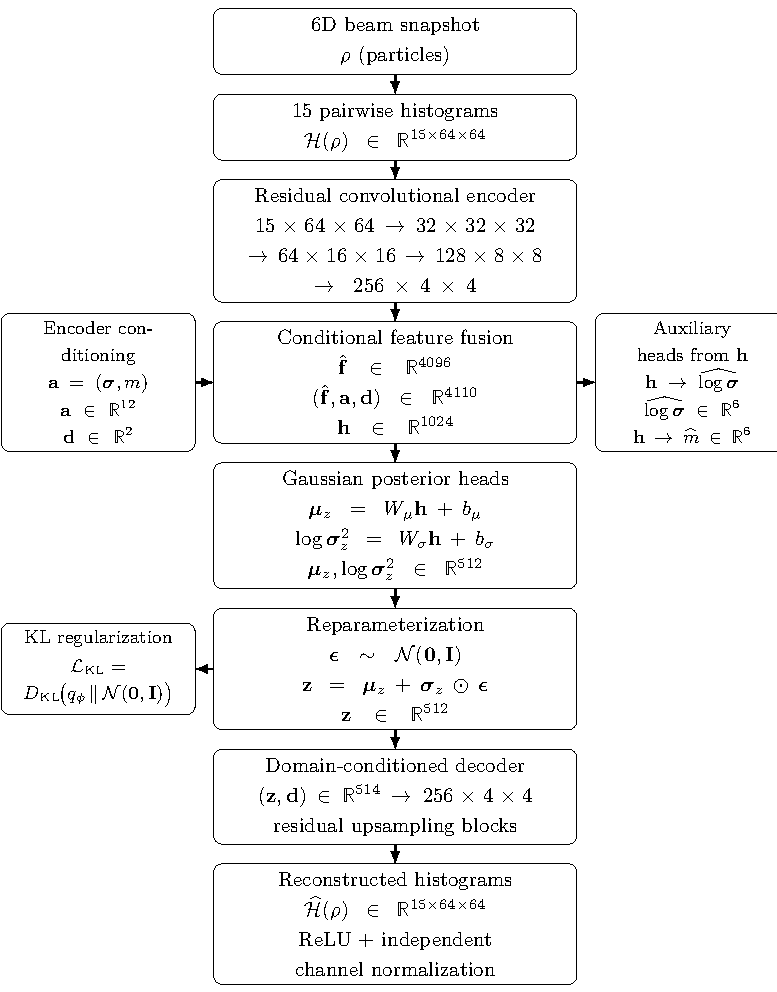
\includegraphics[width=0.8489\linewidth]{cvae_architecture.pdf}
\caption{Implemented conditional variational autoencoder architecture used to construct the reduced representation of six-dimensional beam snapshots.}
\label{fig:cvae_architecture}
\end{figure}

Each particle distribution \(\rho\) is mapped to the complete set of 15 pairwise two-dimensional histograms \(\mathcal{H} ( \rho ) \in \mathbb{R}^{15 \times 64 \times 64} .\) Four residual convolutional downsampling blocks compress this representation to a 256 \(\times\) 4 \(\times\) 4 feature tensor. After flattening, the 4096 convolutional features are concatenated with the 12 auxiliary beam statistics \textbf{a} \(= ( \sigma , m ) \in \mathbb{R}^{12}\) and the two-component domain token d, and projected to a shared feature \textbf{h} \(\in \mathbb{R}^{1024} .\) Two linear heads parameterize a 512-dimensional Gaussian posterior, from which the latent state \textbf{z} is sampled through the reparameterization trick. The decoder receives only the latent state and the domain token, \(( \mathrm{z} ,\) d), and reconstructs the 15 pairwise histograms through residual upsampling blocks. In parallel, two auxiliary heads branch directly from the shared encoder feature \textbf{h} to predict the six logarithmic rms beam sizes and the six phase-space centroids. Each reconstructed histogram channel is constrained to be non-negative and normalized independently over its 64 \(\times\) 64 grid.

The implemented CVAE acts on the full collection of pairwise projected beam densities rather than on a single low-dimensional observable. For a six-dimensional phase-space distribution \(\rho ,\) the preprocessing operator constructs

\[
H(\rho)=\{H_i\}_{i=1}^{15},\qquad H(\rho)\in\mathbb R^{15\times64\times64},
\]

corresponding to the complete set of pairwise two-dimensional projections of the six phase-space coordinates. These 15 histograms are supplied jointly as channels of the convolutional encoder.

The encoder contains four residual downsampling blocks. Starting from the 64 \(\times\) 64 spatial grid, successively downsampling the feature map by a factor of two in each dimension produces the sequence until the final 4 \(\times\) 4 feature map is reached. The channel dimension is simultaneously increased from 15 to 256 through successive convolutional operations.

Each block first applies a stride-two convolution. The resulting feature map is then transformed through group normalization, GELU activation, and a second convolutional operation, with a residual connection around the transformation. The final feature tensor therefore contains 256 \(\times\) 4 \(\times\) 4 \ensuremath{=} 4096 scalar features.

The convolutional representation is conditioned on explicit low-order beam statistics. The auxiliary vector is defined as \textbf{a} \(= ( \sigma , m ) \in \mathbb{R}^{12} ,\)

A two-dimensional domain token \textbf{d} \(\in \mathbb{R}^{2}\) is additionally concatenated with the encoded histogram features. The input to the fully connected fusion layer is therefore

\[ (\widehat f,\mathbf a,\mathbf d)\in\mathbb R^{4096+12+2}=\mathbb R^{4110}.\]

The shared conditioned feature is

\begin{equation}
\label{eq:142}
h=\operatorname{GELU}\bigl(W_h(\widehat f,\mathbf a,\mathbf d)+b_h\bigr),\qquad h\in\mathbb R^{1024}.
\end{equation}

Two independent linear heads parameterize the approximate Gaussian posterior,

\(m_{z} = W_{m} \mathrm{h} + b_{m} ,\) log \(\sigma_{z}^{2} = W_{\sigma} \mathrm{h} + b_{\sigma} ,\)

with \(m_{z} ,\) log \(\sigma_{z}^{2} \in \mathbb{R}^{512} .\)

The corresponding approximate posterior is

\begin{equation}
\label{eq:143}
q_{\phi}(z\mid H(\rho),\mathbf a,\mathbf d)=\mathcal N\bigl(\mathbf m_z,\operatorname{diag}(\boldsymbol\sigma_z^2)\bigr).
\end{equation}

Sampling is performed through reparametrization of the latent state, which allows gradients to propagate through the stochastic sampling operation. The reparameterization is given by (224). The reconstructed channels are explicitly constrained to represent discrete two-dimensional densities. First, non-negativity is imposed through

\begin{equation}
\label{eq:144}
\widetilde H=\operatorname{ReLU}\bigl(\operatorname{Conv}_{1\times1}(f_{\mathrm{dec}})\bigr),
\end{equation}

Each channel is then normalized independently over the spatial grid,

\begin{equation}
\label{eq:145}
\widetilde H_i=\operatorname{ReLU}\bigl(\operatorname{Conv}_{1\times1}(f_{\mathrm{dec},i})\bigr),\qquad i=1,\ldots,15.
\end{equation}

Consequently,

\begin{equation}
\label{eq:146}
\sum_{u,v}\widehat H_i(u,v)=1,\qquad i=1,\ldots,15.
\end{equation}

If the total intensity of a channel becomes numerically negligible during the early stages of training, the implementation replaces that channel by the uniform density \(H_{i}^{b} ( u , v ) =_{64 \times 64}^{1} ,\) which prevents undefined normalization.

In parallel with the variational posterior, two auxiliary regression heads branch directly from the shared conditioned feature \textbf{h} \(\in \mathbb{R}^{1024} .\) Each head consists of two linear layers with a GELU nonlinearity between the two linear layers. It is important to distinguish the fact that the auxiliary physical heads are not functions of the sampled latent vector z. They directly supervise the shared encoder representation \textbf{h} before its projection onto the stochastic latent posterior.

The rms-size head is supervised in logarithmic space,

\begin{equation}
\label{eq:147}
\mathcal L_{\sigma}=\operatorname{MSE}(\widehat{\log\boldsymbol\sigma},\log\boldsymbol\sigma),
\end{equation}

while the centroid head is trained using

\begin{equation}
\label{eq:148}
\mathcal L_{\mathrm{cent}}=\operatorname{MSE}(\widehat{\mathbf m},\mathbf m).
\end{equation}

The complete snapshot-pretraining objective implemented in the notebook is therefore

\begin{equation}
\label{eq:149}
\mathcal L_{\mathrm{CVAE}}=\mathcal L_{\mathrm{rec}}+\beta\mathcal L_{\mathrm{KL}}+\gamma\mathcal L_{\sigma}+\delta\mathcal L_{\mathrm{cent}},
\end{equation}

where KL regularization term is defined in (227) with \(\beta , \gamma ,\) and \(\delta\) tuneable parameters in the present implementation.

The encoder combines these projected distributions with the explicit conditioning vector \textbf{c} \(= [ \sigma , m ,\) d], containing the six rms beam sizes, the six phase-space centroids, and the domain information. The approximate posterior is parameterized through the latent mean \(m_{z}\) and variance \(\sigma_{z}^{2} ,\) and a 512-dimensional latent state is sampled using the reparameterization trick. The conditional decoder reconstructs the 15 pairwise histograms. In the dual formulation, an auxiliary physical-dimensions head predicts \(\{ ( \sigma_{i} b , m_{i} b ) \}_{i = 1}^{6} ,\) providing an explicit representation of physical scale and location in parallel with the histogram-based latent description. Solid arrows denote forward model evaluation, whereas dashed arrows denote conditioning, regularization, or loss pathways.

The resulting architecture separates two complementary descriptions of the beam. The histogram branch represents the distribution through the set of pairwise projected densities,

\[
H(\rho)=\{H_i\}_{i=1}^{15},
\]

which retains non-Gaussian structure, inter-variable dependence, tails, asymmetries, and multimodal features that cannot be summarized by a small set of low-order moments. These projected densities are compressed into a latent variable

\textbf{z} \(\sim q_{\phi}\) (z \(| \mathcal{H} ( \rho ) ,\) c) \(,\)

where the approximate posterior is parameterized as a diagonal Gaussian,

\(q_{\phi} = \mathcal{N} m_{z} ,\) diag \(\sigma_{z}^{2} .\)

Sampling is performed through

\textbf{z} \(= m_{z} + \sigma_{z} \odot \epsilon , \epsilon \sim \mathcal{N} ( 0 , \mathrm{I} ) ,\)

which preserves differentiability of the stochastic latent representation during training.

The explicit conditioning variables are retained outside the histogram representation because the projected densities and the global physical extent of the beam play distinct roles. In the present implementation, the conditioning vector contains the rms beam sizes, the six phase-space centroids, and the domain information,

\(\mathbf c=[\boldsymbol\sigma,\mathbf m,\mathbf d],\)

with

\[
\boldsymbol\sigma=(\sigma_x,\sigma_y,\sigma_\zeta,\sigma_{p_x},\sigma_{p_y},\sigma_\delta),
\]

and

\[
\mathbf m=(\langle x\rangle,\langle y\rangle,\langle\zeta\rangle,\langle p_x\rangle,\langle p_y\rangle,\langle\delta\rangle).
\]

This conditioning allows the encoder to account explicitly for global translation and scale. The decoder receives only \(( z , d ) ,\) absolute position and extension are therefore predicted separately by the physical-statistics head. The auxiliary physical-dimensions branch extends this separation to the subsequent dynamical surrogate. Rather than requiring the latent state alone to preserve the absolute support of each projected distribution, the model predicts

\[
\{(\widehat\sigma_i,\widehat m_i)\}_{i=1}^{6},
\]

in parallel with the latent representation. The resulting dual description therefore distinguishes between the evolution of projected distribution shape and the evolution of its physical extent and location. This is particularly relevant for long-horizon tracking, where a latent model may reconstruct the normalized morphology of a distribution while progressively losing information about its absolute scale or displacement.

The CVAE objective combines reconstruction accuracy with regularization of the stochastic latent space and, when the dual branch is used, supervision of the explicit physical variables. The complete loss function is

\(\mathcal{L}_{\mathrm{CVAE}} = \mathcal{L}_{\mathrm{rec}} + \beta \mathcal{L}_{\mathrm{KL}} + \lambda_{\mathrm{phys}} \mathcal{L}_{\mathrm{phys}} .\)

The Kullback–Leibler contribution,

\(\mathcal{L}_{\mathrm{KL}} = D_{\mathrm{KL}} ( q_{\phi}\) (z \(| \mathcal{H} ( \rho ) ,\) c) \(, \mathcal{N} ( 0 ,\) I)) \(,\)

regularizes the learned representation toward a continuous Gaussian latent space, while \(\mathcal{L}_{\mathrm{rec}}\) constrains the reconstructed pairwise densities and \(\mathcal{L}_{\mathrm{phys}}\) supervises the explicit scale-andlocation branch.

\section{Tokenized latent dynamics}
\label{sec:04_machine_learning_methodology_tokenized_latent_dynamics}

The latent representation reduces the beam state to a vector \(z_{i} \in \mathbb{R}^{d_{z}}\) at lattice element or observation index \(i .\) The goal is then to learn a propagator

\begin{equation}
\label{eq:150}
z_{i+1}=T_{\theta}(z_i,h_i,\mu),
\end{equation}

where \(h_{i}\) is an element token encoding the local lattice element and \(\mu\) contains global parameters. In residual form,

\begin{equation}
\label{eq:151}
z_{i+1}=z_i+\Delta z_i,\qquad\Delta z_i=f_{\theta}(z_i,h_i,\mu).
\end{equation}

This element-indexed formulation describes the computational architecture, not the available supervision. The training archive supplies only the upstream cloud and the final downstream cloud. Consequently, the loss is applied after decoding the final state \(z_{N} ;\) no target \(z_{i}\) or particle cloud is available for 0 \(< i < N .\) The intermediate latent states are therefore internal recurrent states and must not be interpreted as validated physical beam distributions. Testing the operator at arbitrary propagation lengths would require simulator checkpoints and CVAE training data at the corresponding intermediate locations.

\subsection{Element tokenization}
\label{sec:04_machine_learning_methodology_element_tokenization}

Each lattice element is represented by a token containing categorical type information, element length, local optical information, and relevant physical parameters. A general token can be written as

\begin{equation}
\label{eq:152}
h_i=\operatorname{Tok}(\mathrm{type}_i,L_i,k_i,\beta_i,\alpha_i,\mu_i),
\end{equation}

then projected to the latent model dimension through a learned embedding. Tokenization makes the model aware that beam evolution is not a single black-box map, but a composition of local transformations along a lattice.

\subsection{Transformer baseline}
\label{sec:04_machine_learning_methodology_transformer_baseline}

The Transformer baseline processes the element sequence using causal self-attention \cite{vaswani2017attention}. Given token embeddings \(H \in \mathbb{R}^{N \times d} ,\) attention is

\begin{equation}
\label{eq:153}
\operatorname{Attn}(Q,K,V)=\operatorname{softmax}\left(\frac{QK^{\top}}{\sqrt{d_k}}+M_{\mathrm{causal}}\right)V,
\end{equation}

The causal mask prevents dependence on future elements. However, it does not enforce locality, every previous element may still interact with the current one. Thus, the baseline is expressive but may introduce global mixing artifacts when the physical dynamics are dominated by local or near-local transport.

\subsection{Local-window Transformer}
\label{sec:04_machine_learning_methodology_local_window_transformer}

To test the role of locality, a windowed attention mask is introduced by,

\begin{equation}
\label{eq:154}
M_{ij}=\begin{cases}0,&0\le i-j\le w,\\-\infty,&\text{otherwise},\end{cases}
\end{equation}

where \(w\) is the attention window. This architecture preserves causality while restricting information flow to the most recent upstream elements. Empirically, this modification is expected to reduce nonphysical global mixing and to improve stability of long-lattice rollouts.

In the full causal mask, token \(i\) may attend to every preceding token and to itself, while all future positions are excluded. In the local-window variant, the causal constraint is retained but attention is further restricted to the most recent \(W\) positions; the right panel uses \(W =\) 4 only for visualization. The windowed model therefore changes the temporal connectivity of the Transformer rather than merely reducing its size. In particular, the number and width of the Transformer layers may remain unchanged, while the admissible information pathways are constrained to favor local lattice history.

For a sequence of lattice-conditioned latent tokens indexed by \(i = 1 , \ldots , N ,\) the full causal Transformer prevents access to future states while retaining the complete available history. Its additive attention mask may be written as

\[
M_{ij}^{\mathrm{causal}}=\begin{cases}0,&j\le i,\\-\infty,&j>i.\end{cases}
\]



Consequently, the representation associated with the \(i - \mathrm{th}\) lattice position may directly aggregate information from every preceding token. This choice is appropriate when long-range dependencies are expected to remain directly relevant throughout the entire sequence.

\begin{figure}[!htbp]
\centering
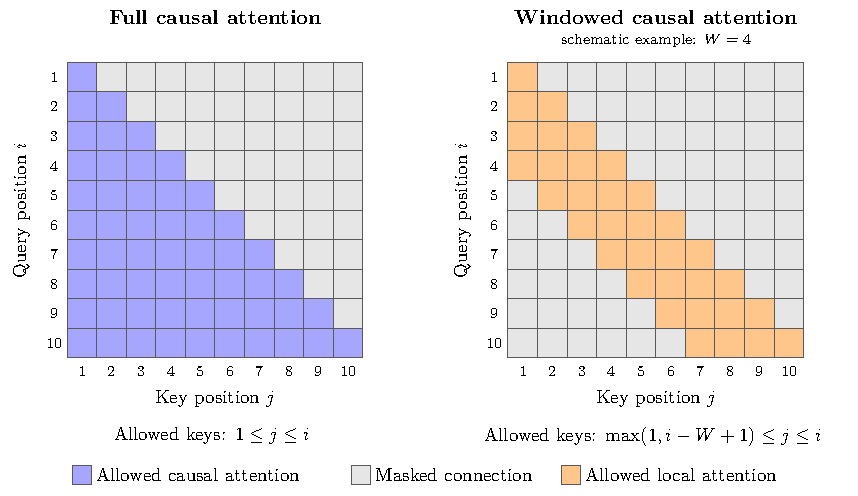
\includegraphics[width=0.9377\linewidth]{causal_and_windowed_attention_masks.pdf}
\caption{Comparison of the attention support used by the full causal and windowed Transformer variants. Rows correspond to query positions \(i\) and columns to key positions \(j .\)}
\label{fig:causal_and_windowed_attention_masks}
\end{figure}

However, for the beam-dynamics problem considered here, the latent evolution is generated through a sequence of local interactions with lattice elements. The full causal mask therefore allows information to propagate along paths that are not physically admissible, which may introduce nonphysical global mixing artifacts.

The windowed variant preserves causality but restricts the admissible support to a local history of width \(W .\) Using the convention that the current token is included in the window, the mask is

\[
M_{ij}^{(W)}=\begin{cases}0,&\max(1,i-W+1)\le j\le i,\\-\infty,&\mathrm{otherwise}.\end{cases}
\]

The direct attention neighborhood of token \(i\) is therefore \(\mathcal{N}_{W} ( i ) =\) \(\{ \mathrm{max} ( 1 , i - W + 1 ) , \ldots , i \} .\) This modification is not equivalent to constructing a smaller Transformer. The window changes the connectivity pattern through which information can propagate. The distinction is therefore one of inductive bias in the learned latent dynamics. In the full causal architecture, the number of directly accessible keys for query \(i\) grows as \(\mathcal{N}_{i} = i ,\) whereas for the local-window mask it is bounded by \(W .\) Thus, the full causal receptive field expands continuously along the lattice, while the windowed attention pattern imposes a fixed local interaction scale at each layer.

The locality constraint does not imply that information older than \(W\) positions is completely inaccessible to a multilayer Transformer. Because the representation produced at one layer already summarizes earlier tokens inside its own local neighborhood, successive layers can propagate information indirectly across a broader range. Ignoring boundary effects, after \(L\) local-attention layers the maximum backward dependency range can grow approximately as \(1 + L ( W - 1 ) ,\) while each individual attention operation remains local. The model therefore retains the possibility of building longer-range dependencies hierarchically, but it must do so through successive local transformations rather than through a single unrestricted attention step.

\subsection{Graph Neural Operator latent propagator}
\label{sec:04_machine_learning_methodology_graph_neural_operator_latent_propagator}

A Graph Neural Operator represents the lattice as a directed graph. Nodes correspond to lattice elements or observation points, and directed edges encode physically admissible interactions. The continuous operator layer

\begin{equation}
\label{eq:155}
v_{\ell+1}(x)=\sigma\left(Wv_{\ell}(x)+\int_{\Omega}K_{\theta}(x,y)v_{\ell}(y)\,\mathrm dy\right)
\end{equation}

is discretized as message passing,

\begin{equation}
\label{eq:156}
v_i^{\ell+1}=\sigma\left(Wv_i^{\ell}+\sum_{j\in\mathcal N(i)}K_{\theta}(h_i,h_j)v_j^{\ell}\right).
\end{equation}

In the beam-dynamics setting, \(\mathcal{N} ( i )\) can be chosen to respect directionality and locality along the lattice. This makes the GNO a natural approximation of a localized transport kernel. It also provides a physical interpretation of why its behavior may resemble that of a local-window Transformer while being more explicitly tied to operator learning and message passing.

\section{Loss functions and validation metrics}
\label{sec:04_machine_learning_methodology_loss_functions_and_validation_metrics}

The snapshot CVAE is pretrained before the latent propagators. Its implemented objective is

\begin{equation}
\label{eq:157}
\mathcal L_{\mathrm{CVAE}}=\mathcal L_{\mathrm{rec}}+10^{-2}\mathcal L_{\mathrm{KL}}+10^{-3}\mathcal L_{\sigma}+10^{-3}\mathcal L_{\mathrm{cent}},
\end{equation}

where \(\mathcal{L}_{\mathrm{rec}}\) is the reconstruction error of the fifteen normalized histograms, \(\mathcal{L}_{\sigma}\) is the mean-squared error of the six logarithmic coordinate-wise RMS spreads, and \(\mathcal{L}_{\mathrm{cent}}\) is the mean-squared error of the six centroids.

For latent propagation, only the final decoded state is supervised. Let \(H_{N , p}^{( s )}\) be target projection \(p\) of sample \(s\) and let \(H_{N , p}^{b^{( s )}} = \mathcal{D}_{\psi} ( z_{N}^{( s )} )\) be the decoded prediction. The endpoint histogram term used in the Transformer window study is

\begin{equation}
\label{eq:158}
\mathcal L_{\mathrm{hist},N}=\frac1{15B}\sum_{s=1}^{B}\sum_{p=1}^{15}\sum_{a,b}\left(\widehat H_{N,p}^{(s)}[a,b]-H_{N,p}^{(s)}[a,b]\right)^2.
\end{equation}

The complete endpoint objective is

\begin{equation}
\label{eq:159}
\mathcal L_{\mathrm{prop}}=\mathcal L_{\mathrm{hist},N}+\beta_{\mathrm{KL}}\mathcal L_{\mathrm{KL}}+10\mathcal L_{\log\sigma,N}+10\mathcal L_{m,N},
\end{equation}

with

\begin{equation}
\label{eq:160}
\mathcal L_{\log\sigma,N}=\operatorname{MSE}(\widehat{\log\boldsymbol\sigma}_N,\log\boldsymbol\sigma_N),\qquad\mathcal L_{m,N}=\operatorname{MSE}(\widehat{\mathbf m}_N,\mathbf m_N).
\end{equation}

The KL weight is selected independently for each Transformer window and is linearly warmed up during the first ten epochs. The pretrained CVAE decoder remains frozen during this sweep, while the convolutional encoder and posterior heads are trainable so that \(\beta_{\mathrm{KL}}\) has a gradient effect. The tokenizer and latent propagator are trained jointly. In the later physical-statistics-head fine-tuning stage, the complete distribution branch is frozen and only the statistics head is optimized. No sum over intermediate physical checkpoints is present in the implemented objective.

Training loss and reported validation metrics are distinct. Each histogram channel is normalized to unit mass, and the reported relative histogram error is the mean relative \(L^{1}\) discrepancy

\begin{equation}
\label{eq:161}
\epsilon_{\mathrm{rel}}=\frac1{15B}\sum_{s=1}^{B}\sum_{p=1}^{15}\frac{\left\|\widehat H_{N,p}^{(s)}-H_{N,p}^{(s)}\right\|_1}{\left\|H_{N,p}^{(s)}\right\|_1+\varepsilon}.
\end{equation}

Because the target channels have unit mass, the denominator is approximately one; the metric measures total absolute probability-mass discrepancy per projection. The other retained metrics are summarized in Table 5.

\begin{table}[!htbp]
\centering\small
\caption{Metrics used for quantitative comparison of surrogate models.}
\label{tab:5}
\begin{adjustbox}{max width=\linewidth}
\begin{tabular}{lll}\toprule
Metric & Symbol & Interpretation\\\midrule
Relative histogram error & $\epsilon_{\mathrm{rel}}$ in Eq.~\eqref{eq:161} & Projected mass discrepancy\\
Mean absolute centroid error & $\|\widehat{\mathbf m}-\mathbf m\|_1/6$ & Centroid accuracy\\
Mean RMS-spread error & $\|\widehat{\boldsymbol\sigma}-\boldsymbol\sigma\|_1/6$ & Coordinate-scale accuracy\\
Wasserstein distance & $W_1(\widehat\rho,\rho)$ & Geometric mass displacement\\
Sliced Wasserstein distance & $\mathrm{SW}(\widehat\rho,\rho)$ & Distributional transport discrepancy\\
Residual bias & $\mathbb E[\widehat H-H]$ & Systematic reconstruction structure\\
Inference time & $t_{\mathrm{inf}}$ & Neural forward-evaluation cost\\\bottomrule\end{tabular}
\end{adjustbox}
\end{table}

\section{Conditional latent uncertainty estimation}
\label{sec:04_machine_learning_methodology_conditional_latent_uncertainty_estimation}

The stochastic latent representation of the CVAE can be propagated through the complete global physical surrogate to obtain an ensemble of predictions for a fixed input beam and fixed machine parameters. This construction is used as a diagnostic of the model’s conditional latent variability. It is important to distinguish this quantity from a complete Bayesian treatment of the model, which would require marginalization over the model parameters \(\theta\) in addition to the latent variable \(z .\) The present approach instead uses the stochastic latent representation to quantify uncertainty in the predicted beam distribution for a fixed trained model. This model does not include uncertainty associated with finite training data, model misspecification, or parameter uncertainty. It is therefore a conditional uncertainty estimate rather than a complete Bayesian posterior.

\section{Posterior sampling and propagation}
\label{sec:04_machine_learning_methodology_posterior_sampling_and_propagation}

For an input histogram representation \(X_{0} = \mathcal{H} ( \rho_{0} ) ,\) and conditioning variables \(c_{0} ,\) the encoder defines

\begin{equation}
\label{eq:162}
q_{\phi}(z_0\mid X_0,c)=\mathcal N\left(\mathbf m_{\phi}(X_0,c),\operatorname{diag}[\boldsymbol\sigma_{\phi}^{2}(X_0,c)]\right).
\end{equation}

An ensemble of \(R\) initial latent states is generated through the reparameterization

\begin{equation}
\label{eq:163}
z_0^{(r)}=\mathbf m_{\phi}(X_0,c)+\boldsymbol\sigma_{\phi}(X_0,c)\odot\epsilon^{(r)},\quad\epsilon^{(r)}\sim\mathcal N(0,I),\quad r=1,\ldots,R.
\end{equation}

The machine parameters \(\mu ,\) lattice tokens \(\{ h_{n} \}_{n = 0}^{N - 1} ,\) and physical conditioning variables are held fixed across the ensemble. Each sample is propagated through the same learned latent dynamics,

\begin{equation}
\label{eq:164}
z_N^{(r)}=\mathcal T_{\theta}^{N}\left(z_0^{(r)},\{h_n\}_{n=0}^{N-1},\mu\right),
\end{equation}

and decoded into the fifteen normalized pairwise histogram masses,

\begin{equation}
\label{eq:165}
\widehat H_{N,p}^{(r)}=D_{\psi}(z_N^{(r)},c_N)_p,\qquad p=0,\ldots,14.
\end{equation}

The global physical model also returns the six predicted RMS extensions and centroids \(\sigma_{N}^{( r )} b\) and \(m_{N}^{( r )} c\) for each sample. These quantities are used to convert the normalized histogram masses into physical densities.

For a pair \(p = ( a , b ) ,\) the normalized histogram mass is converted into a physical density by assigning bin edges from the predicted centroid and RMS extension. If \(\Delta u_{p , i}^{( r )}\) and \(\Delta v_{p , j}^{( r )}\) are the resulting physical bin widths, then

\begin{equation}
\label{eq:166}
\widehat\rho_{N,p,ij}^{(r)}=\frac{\widehat H_{N,p,ij}^{(r)}}{\Delta u_{p,i}^{(r)}\Delta v_{p,j}^{(r)}}.
\end{equation}

Consequently, variability in the physical-density ensemble contains both decoded shape variability and variability introduced by the physical-statistics head.

\subsection{Monte-Carlo estimators}
\label{sec:04_machine_learning_methodology_monte_carlo_estimators}

For any predicted bin quantity \(A_{i j}^{( r )} ,\) representing either normalized mass or physical density, the empirical predictive mean is

\begin{equation}
\label{eq:167}
\overline A_{ij}=\frac1R\sum_{r=1}^{R}A_{ij}^{(r)}.
\end{equation}

The population-form Monte-Carlo variance and standard deviation used in the implementation are

\begin{equation}
\label{eq:168}
s_{A,ij}^{2}=\frac1R\sum_{r=1}^{R}\left(A_{ij}^{(r)}-\overline A_{ij}\right)^2.
\end{equation}

The signed and absolute discrepancies of the ensemble mean with respect to the reference are

\begin{equation}
\label{eq:169}
b_{A,ij}=\overline A_{ij}-A_{ij}^{\mathrm{true}},\qquad e_{A,ij}=\left|\overline A_{ij}-A_{ij}^{\mathrm{true}}\right|.
\end{equation}

Spatial averages, maxima, and sums of these fields are then used to summarize the uncertainty distribution over a selected 64 \(\times\) 64 marginal.

The same estimators are applied to each physical statistic. For coordinate \(d ,\)

\begin{equation}
\label{eq:170}
\overline\sigma_d=\frac1R\sum_{r=1}^{R}\widehat\sigma_d^{(r)},\qquad s_{\sigma_d}^{2}=\frac1R\sum_{r=1}^{R}\left(\widehat\sigma_d^{(r)}-\overline\sigma_d\right)^2,
\end{equation}

with analogous definitions for \(m_{d}\) and \(s_{m_{d}} .\)

Empirical central intervals may additionally be obtained from ensemble quantiles,

\begin{equation}
\label{eq:171}
I_{1-\alpha}(A_{ij})=\left[Q_{\alpha/2}(\{A_{ij}^{(r)}\}_{r=1}^{R}),Q_{1-\alpha/2}(\{A_{ij}^{(r)}\}_{r=1}^{R})\right].
\end{equation}

